\begin{savequote}[75mm]
The purpose of business is changing over time to reflect our desire for companies to contribute to the world.
\qauthor{George Serafeim}
\end{savequote}

\chapter{Introduction}

\begin{keytakeaway}
In this chapter I will introduce the topic of \textbf{decarbonization} and the role of \textbf{corporate emissions} in the process. I will also introduce the main objectives of this research and the motivation behind them.   
\end{keytakeaway}

\section{The Climate Transition}
The world is currently facing an unprecedented climate crisis, with global temperatures rising at an alarming rate and extreme weather events becoming more frequent and severe. The negative externalities of human-induced greenhouse gas emissions are worrying, with the World Health Organization estimating that climate change will be responsible for over 250,000 additional deaths per year between 2030 and 2050 \cite{WHO2023}. There is an urgent need for immediate and sustained action to reduce the negative effects of climate change. To do so, we must transition to a low-carbon economy, by increasing the adoption of renewable energy sources, improving energy efficiency, and promoting sustainable practices. This is one of the most pressing challenges of our time, and it is not an easy task: it requires a concerted effort from governments, businesses, and individuals to reduce greenhouse gas emissions in a race against time, where every second matters \cite{Muryani2023Strategies}.

\section{Companies drive decarbonization}
\noindent The Paris Agreement sets forth ambitious objectives to combat climate change, aiming to cap the increase in global temperatures to 2°C, with an aspirational target of 1.5°C, above pre-industrial levels. This is to be achieved through a series of significant measures, including reaching net-zero greenhouse gas emissions by 2085 and a reduction of these emissions by 10\% by 2030 \cite{Sanderson2016What}. While a great emphasis is often placed on \textit{what} should be changed, it is not always clear \textit{who} should be responsible for these changes. Should it be goverments designing better policies? Should it be consumers demanding more sustainable products? Should it be non-profits and NGOs advocating for change? Should it be the reader (who is very kind in reading this thesis)  turning off the lights when leaving the room? While all of these actors play an important role in the fight against climate change, taking a pragmatic approach, a study from the Carbon Disclosure Project - a leading organization in the field of corporate emissions - shows how about 71\% of global greenhouse gas (GHG) emissions from 1988 to 2015 are linked to just 100 companies \cite{Cdp2017}. So there we have it, we have found our culprits, and we might have also just found our solution. 

The data is clear, most of GHG emissions come from companies' activities and, for this reason, firms are the ones that can make the most significant impact in the fight against climate change. Simply put, we need companies to be the driving force behind decarbonization. Reassuringly, there is an aligment of interests as businesses are governed by executives who live in the same world as the rest of us, and they too are concerned about the future of the planet (albeit some more than others). As Professor Serafeim points out, there is an evolving business paradigm reflecting a collective desire for companies to positively impact the world \cite{purpose+profit}. Consequently, firms are increasingly playing an active role in addressing climate change by setting ambitious emission reduction targets, investing in renewable energy sources, and transitioning towards a low-carbon economy. Most interestingly, companies do not do this only because they are good citizens, but also because they see a business opportunity in the transition to a low-carbon economy. As Gallego-Alvarez et al. argue, a reduction in carbon emissions generates a positive impact on financial performance \cite{Gallego}.
Ultimately, the transition to a low-carbon economy is not to be seen as an inefficiency, but rather a demand for innovation and a source of new business opportunities. By transitioning to a low-carbon economy, companies can create value for their shareholders, employees, and society at large \cite{purpose+profit}. 


\section{The Role of Data}
The transition to a low-carbon economy will have a profound impact on the business world and, when it comes to sustainability, it will require significant changes in the way companies operate, creating both risks and opportunities \cite{purpose+profit}. Companies that are able to reduce their emissions will be better positioned to succeed in the future business landscape, while companies that are unable to do so will face significant risks. 

Inevitably, as in any paradigm shift, there will be winners and loosers. A key question remains, how can we tell them apart? In this context, the role of data becomes crucial. Data serves an internal function, by helping companies understand their climate risk and identify the best strategies to reduce their emissions. At the same time, data also serves an external function, by helping investors allocate their resources more efficiently and policymakers design effective policies. Such role has been recognized by the market, that has been shown to value companies' greenhouse gas emission disclosures, with stock prices reflecting estimates of non-disclosed emissions and a significant market response to climate change information in 8-K filings \cite{Griffin}. Additionally, governments are increasingly interested in regulating data reporting through the implementation of mandatory disclosure requirements. For example the European Union's as of the 5th of January 2023, started enforcing the Corporate Sustainability Reporting Directive (CSRD) which requires companies to disclose their climate-related information. The directive modernises and strengthens the rules concerning the social and environmental information that companies have to report. A broader set of large companies, as well as listed SMEs, will now be required to report on sustainability. Some non-EU companies will also have to report if they generate over EUR 150 million on the EU market \cite{EuropeanCommission2023}. While the European Union is leading the way, other countries are also following suit, with the United States, Switzerland, United Kindgdom, and Canada also implementing similar regulations and with China, India, Israel, and Japan also considering similar measures \cite{Jonson2022}. In line with this global movement, key institutions such as the Carbon Disclosure Project (CDP) are  playing a crucial role in promoting corporate disclosure of climate-related information, driving engagement on environmental issues, and providing a globally consistent disclosure standard for GHG emissions and information on a firm’s activities to reduce carbon emissions \cite{CDP2024}. 





% When it comes to sustainability, the transition will require significant changes in the way companies operate, and it will create both risks and opportunities \cite{purpose+profit}. For instance, companies that are able to reduce their emissions will be better positioned to succeed in the transition, while companies that are unable to do so will face significant risks. The transition will also create opportunities for new business models and technologies, and it will require companies to adapt to new regulations and policies. In this context, it is crucial for companies to understand their climate risk and to identify the best strategies to reduce their emissions and to succeed in the transition to a low-carbon economy. This is where the role of data and modeling techniques becomes crucial. Not only can these techniques help companies understand their climate risk, but they can also help companies identify the best strategies to reduce their emissions and to succeed in the transition to a low-carbon economy. Under this framework, it is therefore not surprising to see that companies are increasingly interested in understanding their climate risk and in identifying the best strategies to reduce their emissions and to succeed in the transition to a low-carbon economy and are increasingly more willing to disclose them.


% These goals require substantial transformations in global economic structures, especially in the areas of energy consumption and the development of renewable energy sources. For instance, in the United States, attaining deep decarbonization necessitates a national overhaul in the way energy is produced and used, with implications for urban planning and land management \cite{Hsu2022Planning}. Similarly, in the European Union, deep decarbonization could be pursued via either a demand-driven system or a centralized approach to manage carbon emissions. However, achieving more ambitious targets will require a broader mix of technologies and greater intersectoral synergy \cite{Korkmaz2020A}. Numerous policy instruments, particularly carbon taxation, are progressively being implemented in major developed economies. Some experts advocate for a global carbon tax as a potent mechanism to expedite decarbonization in the energy sector. However, this approach encounters several hurdles, including substantial capital investment needs, competition between different sectors, varying environmental policies across regions, and the challenge of securing public acceptance for changes in energy consumption habits \cite{Papadis2020Challenges}.


% In my opinion, regardless of the specific outcomes of a global carbon tax, the transition to a low-carbon economy is inevitable and will have a profound impact on the business world. This is because, despite the decrease in 2020 due to the COVID-19 pandemic, global energy-related CO 2 emissions remained at 31.5 Gt, contributing to CO2 reaching its highest ever average annual concentration in the atmo-sphere of 412.5 parts per million in 2020 – roughly 50\% higher than when the industrial revolution began. Global energy-related CO 2 emissions are expected to rebound and continue increasing, as demand for coal, oil, and gas recovers along with the economy \cite{BHATT2023100095}. It seems like carbon emissions are arguably the greatest negative externality that is currently affecting global markets, we don't yet have a single global policy to regulate emissions, that is not game theory optimal for a country to commit to lowering emissions before others, but chances are that if the decabonization strategy is not implemented, the world will face a climate crisis that will have a profound impact on the economy. Interestingly, the more we wait to implement a decarbonization strategy, the more likely it will be that the transition will need to be more abrupt, and in this case firms that are not prepared will face significant risks, while firms that are prepared will have a competitive advantage. As Professor Serafeim argues, such transition should not be seen as an inefficiency, but rather as a demand for innovation and a source of new business opportunities \cite{purpose+profit}. Indeed, by transitioning to a low-carbon economy, companies can create value for their shareholders, employees, and society at large. Therefore, if a company is to succeed in a modern business landscape, it must do so by alignign its profit strategy with a concrete purpose strategy, which includes a commitment to lowering carbon emissions. When it comes to sustainability, the transition will require significant changes in the way companies operate, and it will create both risks and opportunities \cite{purpose+profit}. For instance, companies that are able to reduce their emissions will be better positioned to succeed in the transition, while companies that are unable to do so will face significant risks. The transition will also create opportunities for new business models and technologies, and it will require companies to adapt to new regulations and policies. In this context, it is crucial for companies to understand their climate risk and to identify the best strategies to reduce their emissions and to succeed in the transition to a low-carbon economy. This is where the role of data and modeling techniques becomes crucial. Not only can these techniques help companies understand their climate risk, but they can also help companies identify the best strategies to reduce their emissions and to succeed in the transition to a low-carbon economy. Under this framework, it is therefore not surprising to see that companies are increasingly interested in understanding their climate risk and in identifying the best strategies to reduce their emissions and to succeed in the transition to a low-carbon economy and are increasingly more willing to disclose them.


\section{Carbon Disclosure Project}
% \begin{figure}[H]
%     \centering
%     
\includegraphics[width=0.5\textwidth]{figures/cdp_logo.png}
%     \caption{Carbon Disclosure Project Logo. Adapted from \cite{CDPMain2024}.}
%     \label{fig:my_label}
% \end{figure}

The primary data source for this thesis is the Carbon Disclosure Project (CDP) Climate Change Questionnaire \cite{CDP2024}, which was kindly provided to me by the Climate and Sustainability Impact Lab from the Digital Design Institute at the Harvard Business School \cite{HarvardD3Lab2024}. The Carbon Disclosure Project is a not-for-profit charity that runs the global disclosure system for investors, companies, cities, states and regions to manage their environmental impacts \cite{CDPMain2024}. The importance of the CDP is widely recognized by the business and the academic communities. As Ban Ki Moon, former Secretary General of the United Nations, states ``The work of CDP is crucial to the success of global business in the 21st century... helping persuade companies throughout the world to measure, manage, disclose and ultimately reduce their greenhouse gas emissions. No other organization is gathering this type of corporate climate change data and providing it to the marketplace'' \cite{CDPMain2024}. The Carbon Disclosure Project Sustainability Questionnaire uses the Greenhouse Gas (GHG) Protocol as a reporting model for carbon-related data \cite{Andrew2011Accounting}. It is one of the largest datasets of self-reported GHG emissions and collects a wide range of information on climate change-related topics. The questionnaire provides a globally consistent disclosure standard for GHG emissions and information on a firm’s activities to reduce GHG emissions. The CDP is backed by a large number of institutional investors, including banks, insurance companies, asset management companies, and pension funds holding US\$100 trillion in assets (i.e., CDP signatories), which act as ``norm entrepreneurs'' \cite{OTT201714}. Currently more than 23,000 companies disclose their emission data through the survey, representing two thirds of global market capitalization \cite{CDPMain2024}. 

\subsection{Motivations Behind Corporate Disclosure to the CDP}
The Carbon Disclosure Project (CDP) questionnaire has not only gained increasing popularity among companies but has also become an important tool for investors and other stakeholders in evaluating corporate climate risks. It plays a crucial role in identifying effective strategies for emission reduction and in navigating the transition towards a low-carbon economy. The growth in the completion and publication rates of the CDP questionnaire reflects its importance, with institutional investors exerting a notable influence on climate change disclosure through corporate communication channels \cite{Cotter2012Institutional}. Consequently, the annual increase in the number of companies engaging in disclosure represents a substantial data pool, invaluable for analyzing the decarbonization process and projecting future emission trends. The rationale for companies to disclose varies, encompassing regulatory compliance, investor expectation alignment, reputation enhancement, peer benchmarking, emission reduction opportunity identification, and risk assessment. Furthermore, disclosing to CDP entails two independent steps: the first involves the completion of the questionnaire, while the second involves the publication of the response. The latter step is particularly significant, as it demonstrates a company’s commitment to transparency and accountability, thereby enhancing its reputation and credibility \cite{Cotter2012Institutional}.

\subsection{CDP Scores}
The CDP survey assigns a score (Figure \ref{fig:CDP-scores}) that ranks the performance of companies when decarbonizing.  For reference, 48\% of S\&P companies scored high-performance band B ratings and above in their Carbon Disclosure Project (CDP) reports in 2014 \cite{Upadhyay2022Improving}. When assiging a score, CDP assesses the level of detail and comprehensiveness in a response, as well as the company’s awareness of environmental issues, its management methods and progress towards environmental stewardship \cite{CDP2022ScoringPDF}. Additionally, specifically for climate-change scores, to recieve an A-level grade a copmany must verify at least 70\% of Scope 1, Scope 2 and Scope 3 emissions \footnote{For a detailed breakdown of emission scopes, see Appendix \ref{sec:emission_scopes}} with a CDP-approved verification standard. Among other criteria, to score an A on Climate Change, companies must have robust governance and oversight of climate issues, rigorous risk management processes, verified scope 1 and 2 emissions and be reducing emissions across their value chain. Most Climate Change A List companies as of 2022 have well established emissions targets that have been approved by the SBTi, and evidence of targets which cover their scope 3 emissions \cite{CDP2022ScoringPDF}. The CDP ranking is widely accepted as a benchmark to reflect and review the corporate awareness of environmental challenges, and the best practices for risk mitigation \cite{tefoso}. 


\begin{figure}[h]
    \centering
    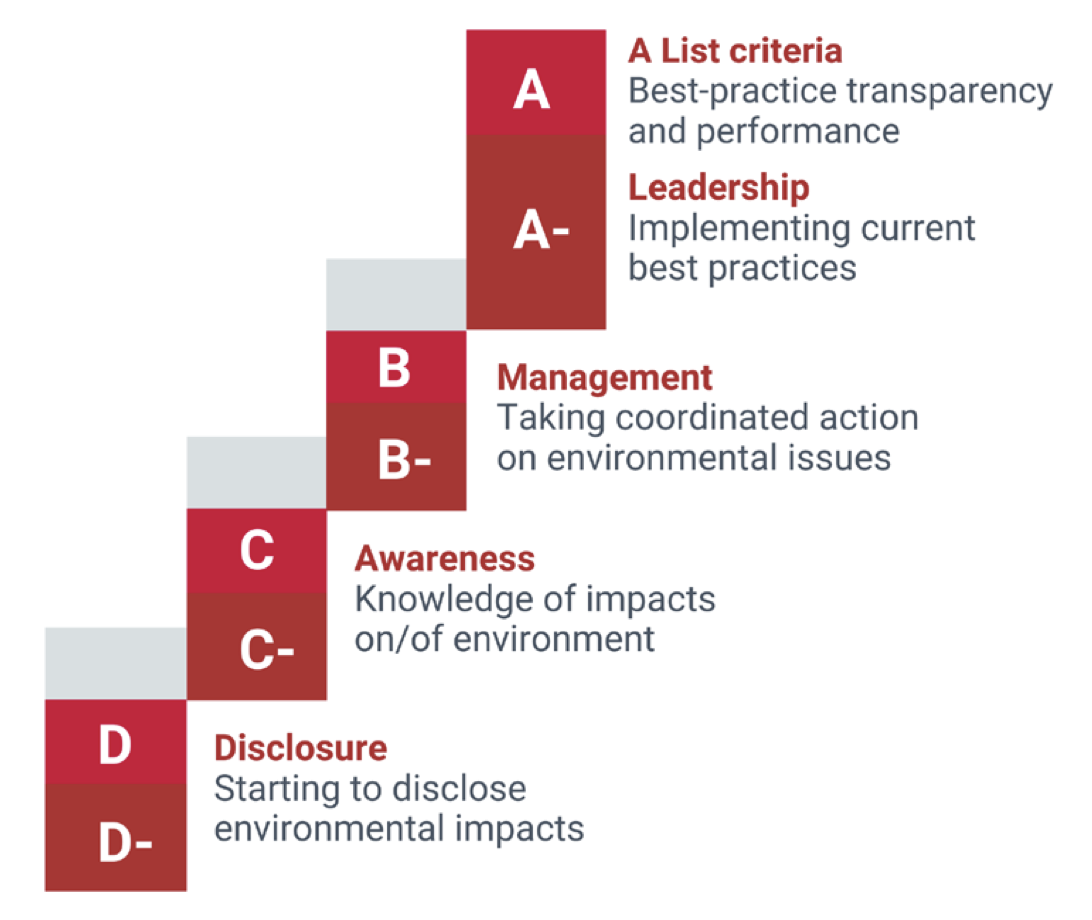
\includegraphics[width=0.6\textwidth]{figures/cdp_scoring.png}
    \caption{Caption of CDP Scoring Grades. Adapted from \cite{CDP2022ScoringPDF}.}
    \label{fig:CDP-scores}
\end{figure}


\subsection{Limitations}


\noindent While the CDP score is a valuable and widely recognized metric, it has several limitations. First, the CDP score is assigned based on adherance to best-practices and does not provide a future outlook on the company-specific ability to reduce emissions. It signals that the company is currently adhearing to best practices, but there is no immediate way to know by how much will the company be able to reduce its emissions in the future. Second, the CDP score is based on self-reported data, which can be subject to biases and errors. Third, the score does not provide an estimate of the company's future emissions, which is crucial for investors and policy makers. Thus, while the score can be useful as a first metric in this thesis we will be experimenting with the data to build more sophisticated models by taking a forward-looking approach to forecasting emissions. That is, we will be looking primarily at Next-Year Decarbonization Rates, which is the percentage change in emissions from one year to the next, and in doing so we will be assessing the predictive power of the CDP data, and which parts of the survey are most useful and correlate with future emissions.

% Here is should add something about the fact that similarly to scores, the CDP data is always used for compliance and never for predictive purposes


% 

\section{Contributions to The Current Literature}
\noindent The literature on decarbonization is vast and covers a wide range of topics, from the impact of climate change on the economy to the role of companies in the transition to a low-carbon economy. In this section, I will focus specifically on the use of modeling based on CDP data and disclosure data to understand what has been done in the past and what are the key questions that remain unanswered. Then, I will use those unanswered questions to motivate the hypothesis and modeling techniques that I will address in this thesis: forecasting next-year decarbonization rates at the company level.


\subsubsection{Current Literature focus is on Estimating Carbon Footprints}
When analyzing the broader literature, the overwhelming majority of studies focus on estimating carbon footprints and emissions rather than forecasting decarbonization rates. Forecasting is a more challenging task, as it requires predicting future emissions based on historical data, and it is very rare to find studies that focus on this specific task. In terms of footprint estimation, Nguyen et al. developed a machine learning model to predict corporate carbon footprints for climate finance risk analyses \cite{nguyen-ml} and found that the best performing models are able to perform some degree of feature selection, as well as boosting and bagging techniques. They find that the Meta-Elastic Net learner combined from multiple well-tuned base-learners is the best performing model \cite{nguyen-ml}. Their research is particularly of interest to us, as they also work with firm-year disclosure data derived in part from the GDP, they use the same industry classification method as this thesis, and they share some predictors with our analysis. The key difference is that our task is analyzing the impact of current corporate actions on future decarbonization, while they are focused on estimating footprint. 


\subsubsection{Forecasting Models focus on aggregated Industry and Country Data}
In terms of pure forecasting models, the literature is primarily focused on country-level or industry-level forecasts, given that the company-level data is not always avaialble, less standardized, and more difficult to work with. For example, in the context of country-level forecasting, the work of Boateng et al. show how Artificial neural network models can be useful for aiding climate change policy decision-making as they effectively predict carbon emission intensity for Australia, Brazil, China, India, and USA with negligible forecasting errors \cite{acheampong}. Predictive models have also been applied to specific countries, such as China with the SSA-LSSVM model by Zhao et al. and the combined MNGM-ARIMA and MNGM-BPNN models by Wang et al. \cite{wangfs, zhaofs}. In the context of industry-level forecasting, Liu et al. use a least squares support vector machine to predict CO2 emissions in China's major industries and residential consumption \cite{liu} or Yang et al. use an ARIMA model to forecast GHG emissions in Shanghai's aviation industry \cite{yang}. 


\subsubsection{The Carbon Disclosure Project data is used for inferencial purposes}
For what regards specifically the use of Carbon Disclosure Project data, the focus is on leveraging CDP data and grades to find relationship with management characteristics and financial performance \cite{nguyen-ml,ben-amar,teob,Hassan2013Carbon}. In this regard, the primary inspiration for this thesis is the work of Lu, Nguyen, and Serafeim who are currently analyzing Incentive Diffusion and Decarbonization rates in the context of the CDP data \cite{incentive-diffusion}. I followed their work closely and used their data as a starting point for my analysis. Furthermore, we both focus on real decarbonization rates - real emission reductions as opposed to emission transfers through acquisitions or divestitures, output-driven emission changes, and accounting-driven emission changes \cite{incentive-diffusion}. The primary difference between their research and mine is that they are focused on understanding the impact of incentives on current decarbonization rates, while I am focused on next-year decarbonization rates. That is, they take an inferential approach testing key hypothesis, while I take a predictive approach, exploring the predictive power of the CDP data and identifying the key predictors of decarbonization rates with a one-year time horizon. 


Another example of using CDP data to address key management questions is the work of Ben-Amar et al. who use CDP data to uncover the relationship between disclosure and board female representation \cite{ben-amar}. In terms of CDP scores, Adel et al. find that firms with higher CDP scores have higher financial performance and better management of greenhouse gas information \cite{teob}. They also find that firms with higher CDP scores are more likely to have a higher level of board diversity, which is associated with better management of greenhouse gas information. Additionally, Hassan et al. study the relationship betweem CDP scores and the UK FTSE top 100 companies disclosure performance \cite{Hassan2013Carbon} .


Overall, \textbf{no one has yet focused on forecasting real decarbonization rates at the company level}, an area still largely unexplored in research. This gap is crucial, as I believe that understanding the effects of current corporate actions on future decarbonization rates is vital for creating better disclosure methods and identifying which companies are best positioned for the transition to a low-carbon economy. The opportunity to base our analysis on CDP data, the largest dataset of self-reported greenhouse gas emissions, offers a unique chance for advancement in this field and for evaluating the variables that will have the most significant impact in terms of future results, and not just in terms of current compliance. 

\section{Motivation}
TODO: This section is mostly to rewrite, introducing the key questions that I will address in the results. 
\subsubsection{Questions}
 Can quantiative forecasting play a central role in enhancing our understanding of global emissions? Will it allow us to make strategic decisions when decarbonizing? Can we build a more sustainable future with a targeted approach that uses data to identify potential for improvement? What other data do we need to increase our prediction accuracy and understend the impact of business strategies on decarbonization? Can we predict future decarbonization rates and, if so, what is the best way to do it? \\ 
 \subsubsection{Why is this important? and the interesection of academic and business interest}
 \noindent Those are only a few of the very important and interesting questions that drew me to research decarbonization and to focus on the role of corporate emission-level data in the process. I believe that research in this area is crucial to advance our ability to build a more sustainable future. Furthermore, the answers to these questions can help us make better decisions and build a more sustainable future while also creating value for businesses. Additionally, the call for more data in decarbonization comes not only from the academic world but also from the fact that many business opportunities arise from the climate transition that inevitably requrie good and valid information to determine which companies and sectors are winners and loosers, which are the champions in the decarbonization process, which are the laggards, and which are the companies that are greenwashing. I believe that studying specifically corporate emissions and forecasting decarbonization rates as I am doing in this thesis can be useful to three key stakeholders: 
 \subsubsection{The key stakeholders}
 \begin{enumerate}
    \item \textbf{Investors} who are increasingly interested in understanding the climate risk of their portfolios and in identifying the companies that are best positioned to succeed in the transition to a low-carbon economy. For examples, companies such as BlackRock [insert quotation here] are enhancing their sustainable investing strategies and offering more sustainable investment products to their clients.
    \item \textbf{Companies} who are increasingly interested in understanding their climate risk and in identifying the best strategies to reduce their emissions and to succeed in the transition to a low-carbon economy. Additionally, companies might be interested in benchmarking against their peers in the sector to understand how they are performing relative to their competitors and to identify the best practices. 
    \item \textbf{Policy makers} who are increasingly interested in understanding the climate risk of their countries and in identifying the best strategies to reduce their emissions and to succeed in the transition to a low-carbon economy. A sector and company level analysis can be useful in determining optimal targets for new policies, identifying the best practices, and understanding the impact of new policies on the sector and on the economy.
\end{enumerate}

\subsubsection{Connection between computer science and decarbonization}
\noindent Finally, I believe that the use of data and modeling techniques  can help us build a more sustainable future in a practical, nonpolitical, and unbias way. Estimating emissions is an amazing example of how Computer Sicence and Statistical models can help us achieve real impact driving strategic decisions. I argue furthermore that it is only through a quantitative driven approach that we can dimistify the climate debate and make progress in the climate transition. I am confident that work in the modeling decarbonization has an incredible potential to create value for business and society and especially with increasing data availability and computational power, the time is ripe to make progress in this area. As I will explain in the next sections, this thesis is only possible thanks to incresased data availablity and to the willingness of corporates to disclose their emissions.



